\section{Evaluation}\label{sec:evaluation}

We tested the approach with a working prototype and treat the results as
proof-of-concept evidence for a research direction, not as a field result. The
comparison is against a re-implementation of \textsc{AirBugCatcher}'s reproduction
strategy~\cite{airbugcatcher2024}: bounded enumeration of suspect-packet
combinations up to three packets, in order of proximity to the crash, one
attempt per candidate, accepting the first candidate whose crash carries the
expected signature. It is our reading of the published method, not the authors'
tool, and it runs with no trial-time budget, so it enumerates more candidates
than the original would. Both tools face the same simulated device and channel,
so a difference between them is a difference between the two strategies
\emph{under our noise model}; Section~\ref{ssec:eval-noise} measures how much of
the difference the model itself contributes.

Every arm is scored by the same rule. A campaign is a \emph{genuine} reproduction
if the arm credited a recipe \emph{and} that recipe crashes the target with the
channel switched off, a ground truth the tools never see; it is a \emph{false
credit} if the arm credited a recipe that does not. A recipe the tool returns but
declines to validate counts for neither. The \emph{size gap} is the mean number of
packets a genuine recipe carries beyond the true minimum, and \emph{reads} counts
device attempts per campaign. A third arm, the baseline with one confirming
re-run before it credits a candidate, is the confirmation control; its reads are in
Table~\ref{tab:headlines}.
Table~\ref{tab:headlines} summarises the results.

\begin{table*}[!t]
\renewcommand{\arraystretch}{1.3}
\caption{Main results on the same simulated channel. Size gap is the mean extra
packets over the true minimum, over genuine reproductions only; the best value of
each scored column within a benchmark is in bold. RDD's synthetic false credit is one
campaign in 75,000, which rounds to 0.000.}
\label{tab:headlines}
\centering
\begin{tabular*}{\textwidth}{@{\extracolsep{\fill}}l l c c c c@{}}
\toprule
Benchmark & Configuration & Genuine $\uparrow$ & False credit $\downarrow$ & Size gap $\downarrow$ & Reads\\
\midrule
Real head-to-head            & \textsc{AirBugCatcher}                & 0.759 & 0.137 & 0.483 & 9\\
{\footnotesize 6 bugs, 336 campaigns} & \textsc{AirBugCatcher} $+$ 1 confirmation & 0.708 & 0.006 & 0.931 & 24\\
                             & RDD                                   & \textbf{0.848} & \textbf{0.000} & \textbf{0.117} & 45\\
\addlinespace
Resilience at scale          & \textsc{AirBugCatcher}                & 0.266 & 0.632 & 0.518 & 41\\
{\footnotesize 15,000 bugs, 75,000 campaigns} & \textsc{AirBugCatcher} $+$ 1 confirmation & 0.359 & 0.090 & 0.922 & 342\\
                             & RDD                                   & \textbf{0.824} & \textbf{0.000} & \textbf{0.206} & 143\\
\bottomrule
\end{tabular*}
\end{table*}

\subsection{Real bugs, head to head}

The evaluation uses six controller bugs, labelled A--F, in the Zephyr Bluetooth
Low Energy stack compiled for Zephyr's host-native \texttt{unit\_testing} target.
One is a disclosed vulnerability with a CVE identifier, a division by zero in
connection-parameter handling; the other five are reachable controller faults
exercised through harness patches on the same vulnerable controller, one of them
sharing the first bug's binary. Each bug has a fixed window of eight (A, B) or
five (C--F) packets whose minimal recipe has one or two packets, so the
enumeration baseline reaches every true minimum within its first six candidates
when the channel lets it; the difficulty of these bugs lies in the noise, not in
the search. The committed crash dump of bug B carries no backtrace, which makes
exact matching stronger on B than elsewhere.

Through the full pipeline (a synthesised fuzz trace, a crash-grouping front end given to both tools, which is
our deterministic matcher, then each bug's fixed window and either minimiser), RDD
recovers 0.848 of reproductions with no false credit in 336 campaigns; the
baseline recovers 0.759 with 0.137 false credit. % headtohead.json
Over the eight runs RDD spans $[0.76, 0.90]$ and the baseline $[0.67, 0.81]$,
paired per run. RDD's recipes are also tighter: 0.12 extra packets against 0.48,
and 0.89 of them exactly minimal. Both tools suffer the shared front end, which
sometimes assigns a trace to the wrong bug; on correctly grouped traces the rates
are 0.920 and 0.824. Reduced directly from each bug's window on the truth-table
oracle over thirty runs, RDD recovers 0.933 against the baseline's 0.867
(false credit 0.089). % anchor.json
The cost is reads: about 45 device attempts per campaign against 9, spent on the
sequential test's repeated trials; escalations to the language model are identity
checks on attempts already made, not extra reads.

The baseline's false credit is a consequence of accept-first: it books the first
candidate whose crash carries the expected signature, and under our channel a
non-reproducing candidate occasionally does. One confirming re-run removes almost
all of it (0.137 to 0.006) at 24 reads, but costs recall (0.708) because a true
reproduction must now survive both the channel and exact matching twice. RDD produced no false credit in these 336 campaigns, in the 180 truth-table campaigns
on A--F or in the 30 on the suppressor (95\,\% upper bounds on its rate 0.9\,\%,
1.7\,\% and 10\,\%), and one in the 75,000 synthetic campaigns of
Section~\ref{ssec:eval-scale} (a rate of $1.3\times10^{-5}$; upper bound 0.006\,\%). The tool's property is the
$\alpha$-bounded rate of Section~\ref{sec:our_approach}; zero is the measured outcome.

On the real suppressor bug, where a later packet hides the crash (its harness prints
no backtrace, so the target emits bug A's dump), the baseline
recovers 0.875 with 0.125 false credit; RDD recovers every one of the eight
head-to-head campaigns, and 0.9 of the thirty truth-table runs, with no false credit
in either;
bare delta debugging, started from the non-crashing full window, returns nothing,
which is the cost RDD's own choice of \texttt{ddmin} would incur without its
starting-window search (Section~\ref{ssec:eval-levers}).

\subsection{How much is the noise model}\label{ssec:eval-noise}

Two assumed models drive the comparison: the channel's phantom crashes (a
non-reproducing recipe reported as crashing with the target's own dump, 0.02 to
0.07 per attempt), and the crash-report variation applied to every observed crash
(Section~\ref{sec:our_approach}). Table~\ref{tab:noise} repeats the thirty-run
truth-table experiment with each switched off.

\begin{table}[!t]
\renewcommand{\arraystretch}{1.2}
\caption{The six real bugs, thirty runs each, under weaker noise models. Cells are
genuine / false credit over 180 campaigns, so a rate carries a standard error of
about 0.02; reads for the last row are given in the text.}
\label{tab:noise}
\centering
\footnotesize
\setlength{\tabcolsep}{3pt}%
\begin{tabular}{@{}lccc@{}}
\toprule
Noise model & Baseline & $+$ 1 confirmation & RDD\\
\midrule
as committed            & 0.867 / 0.089 & 0.761 / 0.006 & 0.933 / 0.000\\
report variation off    & 0.911 / 0.067 & 0.911 / 0.000 & 0.928 / 0.000\\
phantom crashes off     & 0.933 / 0.000 & 0.750 / 0.000 & 0.933 / 0.000\\
both off                & 0.978 / 0.000 & 0.933 / 0.000 & 0.928 / 0.000\\
\bottomrule
\end{tabular}
\end{table}

The baseline's false credit vanishes exactly when phantom crashes do, and its
recall gap closes when report variation does; with both off it recovers 0.978
with no false credit at about ten reads per campaign, ahead of RDD's 0.928 at
about 47. RDD's results are almost invariant to the two models because the
sequential test absorbs the phantoms and the identity layer absorbs the
variation, which is what they were built for. The comparison is therefore a
statement about the noise the medium is assumed to produce: where a device
reports spurious crashes of the target signature or garbles its reports, RDD
recovers more at higher cost; where it does neither, plain enumeration is the better tool, and a confirming re-run
buys the same recall as RDD at about a third of its reads.

\subsection{Resilience at scale}\label{ssec:eval-scale}

Because only a handful of real emulable bugs exist, we probe robustness with a
synthetic corpus anchored to the real target: fifteen thousand bugs across six
regimes (standard, high-cardinality, suppressor, far-trigger, deep-noise, and
wide-window), 75,000 campaigns per tool. The regimes were chosen by us to stress
structures known to trouble the two search strategies: large input spaces,
non-monotone suppressors, awkward trigger positions, and noise deep enough to push
a true reproduce rate into the SPRT's indifference zone; only the last stresses
RDD. About a third of the population (0.79 in high-cardinality, 0.24 to 0.27
elsewhere) has minimal recipes larger than the baseline's three-packet cap and is
unreachable for it by construction. At this scale the identity layer's second tier
is a rule that accepts a report containing the target's crash-site symbol or
file; it uses the target's known site, so it stands in for the judge's recall
rather than bounding it, and the sweep runs with no model.

RDD averages 0.824 genuine recovery with one false credit in 75,000 campaigns, a
five-packet sub-recipe of a six-packet minimum in the suppressor regime; the baseline averages
0.266 with 0.632, and with one confirming re-run 0.359 with 0.090 at 342 reads
per campaign, because confirmation removes the phantom stop that ended its
campaigns early (Fig.~\ref{fig:regimes}). % resilience.json OVERALL
Each campaign draws its own noise stream, and the bootstrap intervals resample bugs,
not campaigns, since a bug's five campaigns are correlated: RDD $[0.820, 0.829]$, baseline $[0.261, 0.272]$. They quantify
sampling error over our generator, not agreement with real bugs. RDD's reads are
roughly 143 per campaign against the baseline's 41.

\begin{figure}[!t]
\centering
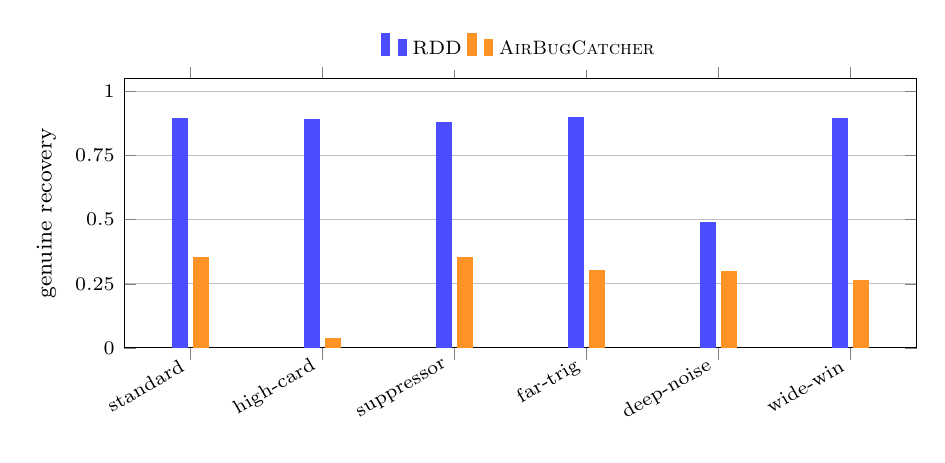
\begin{tikzpicture}
\begin{axis}[
  width=0.96\columnwidth, height=5.0cm,
  ybar, bar width=5.5pt,
  ymin=0, ymax=1.05,
  ylabel={genuine recovery},
  ylabel style={font=\footnotesize},
  symbolic x coords={standard,high-card,suppressor,far-trig,deep-noise,wide-win},
  xtick=data,
  x tick label style={rotate=30,anchor=east,font=\scriptsize},
  ytick={0,0.25,0.5,0.75,1.0},
  yticklabel style={font=\scriptsize},
  legend style={at={(0.5,1.03)},anchor=south,legend columns=2,font=\scriptsize,draw=none},
  enlarge x limits=0.1,
  ymajorgrids,
]
\addplot+[fill=blue!70,draw=blue!70] coordinates {(standard,0.896)(high-card,0.891)(suppressor,0.879)(far-trig,0.897)(deep-noise,0.490)(wide-win,0.893)};
\addplot+[fill=orange!85,draw=orange!85] coordinates {(standard,0.351)(high-card,0.037)(suppressor,0.352)(far-trig,0.300)(deep-noise,0.296)(wide-win,0.261)};
\legend{RDD, \textsc{AirBugCatcher}}
\end{axis}
\end{tikzpicture}
\caption{Genuine recovery per regime (12,500 campaigns each). RDD stays above 0.87
except in deep-noise (0.49, the SPRT indifference zone); the baseline is worst on
high-cardinality inputs, most of which exceed its cap.}% resilience.json per-regime point estimates
\label{fig:regimes}
\end{figure}

The regimes separate the mechanisms. The baseline does best in the standard and
suppressor regimes (0.351, 0.352) and fails almost completely on high-cardinality
inputs (0.037). RDD stays between 0.88 and 0.90 everywhere except deep-noise, where
it drops to 0.490: at that severity the per-attempt reproduce rate of a true
recipe falls to 0.23--0.45 for four fifths of the bugs (0.36 at the modal severity),
inside the indifference zone $(p_0, p_1) =
(0.05, 0.55)$, so the truncated test mostly ends inconclusive, which the tool
scores as a non-reproduction rather than a credit. Its recipes there are no
tighter than the baseline's (0.66 against 0.65 extra packets). Narrowing the band
or raising the trial budget reduces the zone at the price of more reads; RDD
accepts the lost recall to keep the false-credit bound, which is the purpose of
the gate.

\subsection{Where the advantage comes from}\label{ssec:eval-levers}

RDD has several components, and Table~\ref{tab:levers} adds them one at a time
on the real bugs, reducing each bug directly from its window without the shared
front end of Table~\ref{tab:headlines}. These are 48 campaigns (six bugs, eight
runs), so the baseline's recall is 0.771 here (live binary, eight runs) against 0.759 through
the front end and 0.867 on the truth table; its per-run range is $[0.67, 1.00]$.

\begin{table}[!t]
\renewcommand{\arraystretch}{1.2}
\caption{Each component's contribution on the real bugs; each row adds one. The
oracle removes false credit, the identity layer restores recall, the minimiser
survives the suppressor.}
\label{tab:levers}
\centering
\setlength{\tabcolsep}{4pt}%
\begin{tabular}{@{}lccc@{}}
\toprule
 & Genuine & False credit & Genuine\\
Configuration & (A--F) & (A--F) & (suppressor)\\
\midrule
\textsc{AirBugCatcher} baseline    & 0.771 & 0.188 & 0.875\\
$+$ SPRT oracle                    & 0.688 & \textbf{0.000} & 0.000\\
$+$ two-tier identity              & \textbf{0.917} & 0.000 & 0.000\\
$+$ robust minimiser (full RDD)    & 0.917 & 0.000 & \textbf{1.000}\\
\bottomrule
\end{tabular}
\end{table}

Replacing accept-first enumeration by the sequential oracle and \texttt{ddmin}
brings false credit from 0.188 to zero, and it stays there as the other
components are added. % levers.json oracle_fc_invariance
This step changes two things at once, the oracle and the search, so we attribute
to it only the false-credit result; its effect on recall (0.771 to 0.688, per-run
range $[0.33, 1.00]$) is within run-to-run variation. On the suppressor bug it
scores zero, because \texttt{ddmin} bails on a masked full window. Replacing the
exact matcher by the two-tier identity raises recall from 0.688 to 0.917
(+0.229), the largest single gain, and it is a gain against the modelled report
variation of Section~\ref{ssec:eval-noise}. The robust minimiser changes nothing
on the monotone bugs and takes the suppressor from zero to every campaign, by
finding a suppressor-free starting window where plain \texttt{ddmin} finds none.

\subsection{Threats to validity}

\textbf{The simulator.} The device is a deterministic host build of the Zephyr
controller; the channel is a Gilbert--Elliott burst process whose miss rate,
0.44, is our choice rather than a wireless measurement (it lies in the upper
range of the per-test failure frequencies of a flaky-test rerun
corpus~\cite{flakeflagger2021}) and whose phantom rates are ours; the
crash-report variation is a model with rates we chose (backtrace
truncation 0.35, top-frame loss 0.20, frame churn 0.15, log interleaving 0.40,
severe garbling 0.08). Section~\ref{ssec:eval-noise} shows that the headline
advantage is a consequence of these models. A phantom crash is modelled as
carrying the target's own signature, the case that defeats exact matching; a
device that phantoms other crashes, or none, would favour the baseline. RDD
resets the session before every attempt, which in the simulator makes attempts
independent; the burst structure therefore never affects RDD, and the effect of
correlated attempts, which violate the sequential test's precondition, is not
evaluated.

\textbf{The baseline.} It is our re-implementation of one published strategy at
a fifth to a quarter of RDD's reads. The confirmation control shows that one confirming
re-run removes almost all of its false credit; a budget-matched variant with a
different search was not run.

\textbf{Identity.} The deterministic matcher was calibrated post hoc on the same
six bugs (360 same-bug and 360 different-bug pairs generated by the variation
model, no held-out set). The judge accepted every one of the 40 different-bug
pairs the cascade escalates to it and every one of the 57 same-bug pairs, so the
cascade rejects a different-bug report only when the matcher scores it below the
escalation floor, which covers about half of the different-bug pairs in the
calibration set. No experiment here presents a different bug's report to the
in-loop oracle, because each harness emits only its target's crash; the resulting
risk, crediting a recipe that reproduces a different bug, is unmeasured. The
judge's verdicts are replayed from a committed cache; live inference is not
guaranteed bit-reproducible, although re-judging all 386 cached pairs with the
same model tag (Ollama 0.34.2, 24 September 2026) returned every verdict
unchanged.

\textbf{Construct.} ``Genuine'' is defined against a channel-off run of a
deterministic binary. A bug that appears only with channel noise is scored as a
non-reproduction, a bias that trades recall for the false-credit bound; the
truncated test's forced ``no'' is the mechanism we expect behind most of RDD's
deep-noise loss. The code carries an
optional identity guard for binaries that ship several bugs; it is off in every
reported run. Six bugs, one stack, one CVE and one synthetic fault mechanism bound
what the numbers can say.

\subsection{Proposed experiments}

The results order the research plan. First, measure the two assumed rates on a
real link: replay recovered recipes over a software-defined radio and record how
often a non-reproducing recipe crashes the device, with which signature, and how
often the same crash is reported differently; the noise-sensitivity table then
becomes a prediction. Second, present different-bug reports to the in-loop oracle,
on a binary that ships several reachable bugs in one window, and measure
cross-bug credit. Third, run correlated attempts, with reset and settling
disabled, to find the burst regime at which the sequential test's error bound
fails. Fourth, repeat the study on other Bluetooth, Wi-Fi and cellular stacks
using public fuzzing logs, with the matcher's threshold calibrated on held-out
bugs. Fifth, replace the single judge by a calibrated panel evaluated against
human agreement (Cohen's $\kappa$~\cite{cohenkappa1960}), since a judge that never
rejects adds recall but no discrimination. The indifference zone remains; an
adaptive trial budget that spends reads only in the noisiest cases is the
mitigation to test.
